\documentclass{article}

\usepackage{polyglossia}
	\setmainlanguage{german}
\usepackage{amsmath}
\usepackage{siunitx}
    \usepackage{xcolor}
\usepackage{listings}
    \lstset{language=Python}
    \lstset{basicstyle=\footnotesize\ttfamily,breaklines=true}
    \lstset{framextopmargin=50pt,frame=bottomline}
    \lstset{backgroundcolor=\color{white!80!black}, commentstyle=\color{blue}}
\usepackage[margin=4cm]{geometry}
\usepackage{booktabs}
\usepackage{graphicx}
\usepackage{amssymb}

\title{Computational Physics - Exercise 1}
\author{Maurice Donner \& Lukas Häffner}

\begin{document}

\maketitle
\newpage

\section*{Exercise 4 - Numerical Simulation of the 2-Body Problem}
\subsection*{a)}

Every higher order Differential equation can be seperated into a system of
first order Differential equations. We are aiming to use this fact to make
use of the Euler-forward algorithm later. Our ODE looks like this:
    \texttt{Hallo test >> Test "geht das auch nocoh"} 
\[ 
    m_1 \cdot \ddot{\mathbf{x}}_1 = \frac{G m_1 m_2}{\mathbf{r} ^2}, \quad
    m_2 \cdot \ddot{\mathbf{x}}_2 = \frac{G m_1 m_2}{\mathbf{r} ^2}
\]
With \( \mathbf{r} = \big( x_b - x_a, y_b - y_a, z_b - z_a \big) \) being the
relative position of the two bodies \( M_a \ \text{and} \  M_b \).
The Euler algorithm approximates \( x ( t + \Delta t) = x(t) + \Delta t \cdot F(x,t) \)
. The problem now is, that we don't know \( F(x,t) \) yet. All we know is, that
\[ 
    \dot{\mathbf{x}}= \mathbf{v} \quad \& \quad \dot{\mathbf{v}}= F(x,t)
\]
 With \( F_i(x,t) \) being \( G \frac{m_1 m_2}{m_i \mathbf{r}^2 }  \) \\

Looking only at the \( x\)-coordinate, 
we have to fill the following information into the euler algorithm:
 \[ 
     \begin{array}{lcr}
	 x(t + \Delta t) & = & x(t) + \Delta t \cdot v \\ 
	 v(t+\Delta t) & = & v(t) + \Delta t \cdot F(x,t) \\
	& = & v(t) + \Delta t \cdot \frac{F_i}{M_i} 
     \end{array}
 \]
 \begin{lstlisting}[language=python]

    # Define Force
    
    fx = -G*Ma*Mb/absr3*rx
    fy = -G*Ma*Mb/absr3*ry
    fz = -G*Ma*Mb/absr3*rz

    # Update the quantities of Ma

    vxb += fx*dt/Mb
    vyb += fy*dt/Mb
    vzb += fz*dt/Mb

    xb += vxb*dt
    yb += vyb*dt
    zb += vzb*dt

    # Update the quantities of Mb (force acts in the other direction)

    vxa += -fx*dt/Ma
    vya += -fy*dt/Ma
    vza += -fz*dt/Ma

    xa += vxa*dt
    ya += vya*dt
    za += vza*dt

    t += dt
 \end{lstlisting}
 
 \newpage
 Let's throw in some starting values! We set \( M_a = M_b = G = 1 \),
 \( \mathbf{v} _1 = \big( \frac{1}{2} , - \frac{1}{2}, 0 \big) \) and 
 \( \mathbf{v} _2 = \big( - \frac{1}{2} ,  \frac{1}{2}, 0 \big) \). For the
 time step size we choose \( \Delta t = 0.01 \) and the simulation time 
 \( t _{\ \text{sim} } = 100 \), which results in

 \begin{figure}[ht]
     \centering
     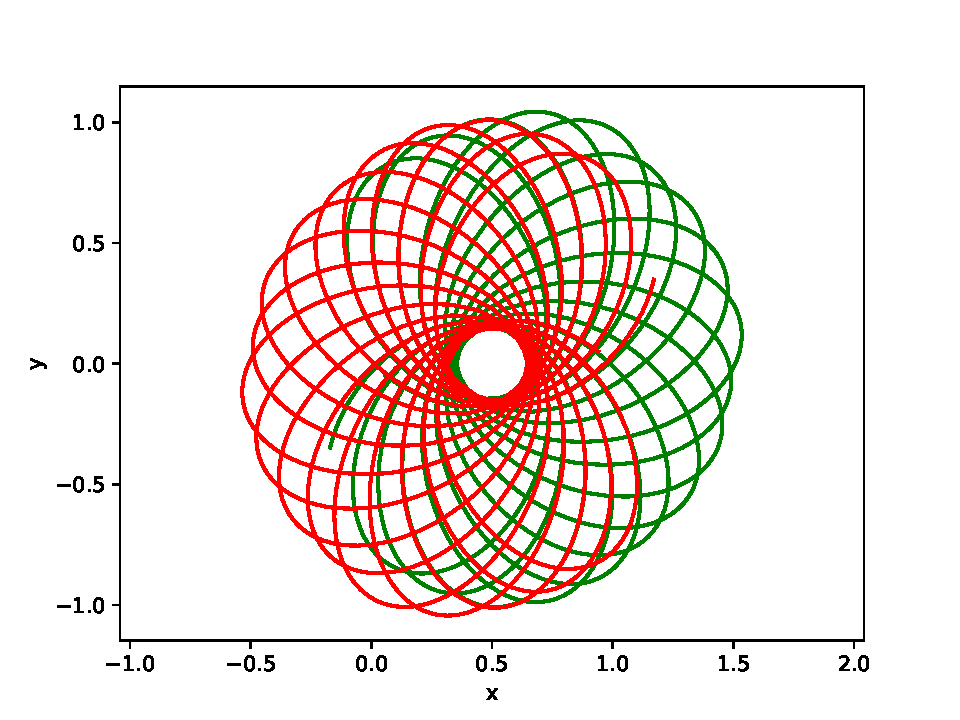
\includegraphics[width=6.5cm]{rosette.pdf} 
     \caption{Trajectories of two Particles with equal mass, approximated} 
 \end{figure}

 \subsection*{b)}

 Now we tackle the question of how to get orbit each other in a perfect circle.
 The needed starting values can be calculated by setting gravitational
 acceleration and Zentripetal acceleration equal:
 \[ 
     \frac{v ^{2}}{R} = G \frac{M_1}{(2R)^2}.
 \]
 The distance between the particles is 1, hence \( R = 0.5 \), so that
 \[ 
     v= \sqrt{G \frac{M_1}{4R} } = \frac{1}{\sqrt{2}} 
 \]
This will force the particles onto a perfectly circular orbit:

\begin{figure}[ht]
    \centering
    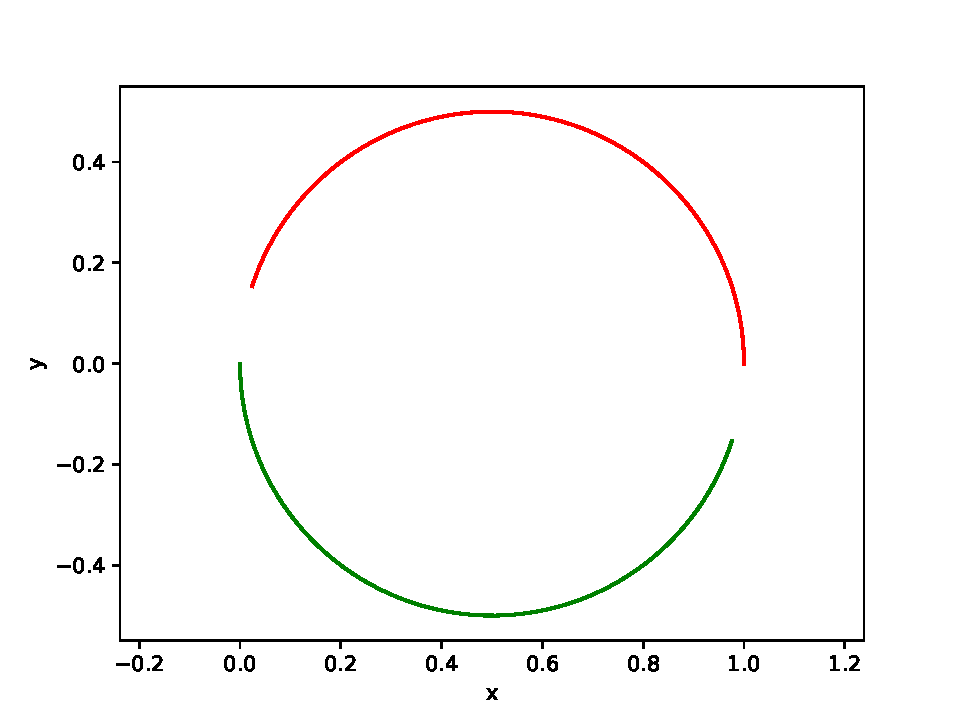
\includegraphics[width=6.5cm]{kreis.pdf} 
    \caption{Particles orbiting each other in a perfect circle}  
\end{figure}

\subsection*{c)} 

If we decrease the velocity from b) by a factor \( \frac{1}{\sqrt{2}} \) the 
orbits of the particles will offset in x-Direction, and the perfecty circular
orbit will become an ellipse-like shape.
\begin{figure}[ht]
    \centering
    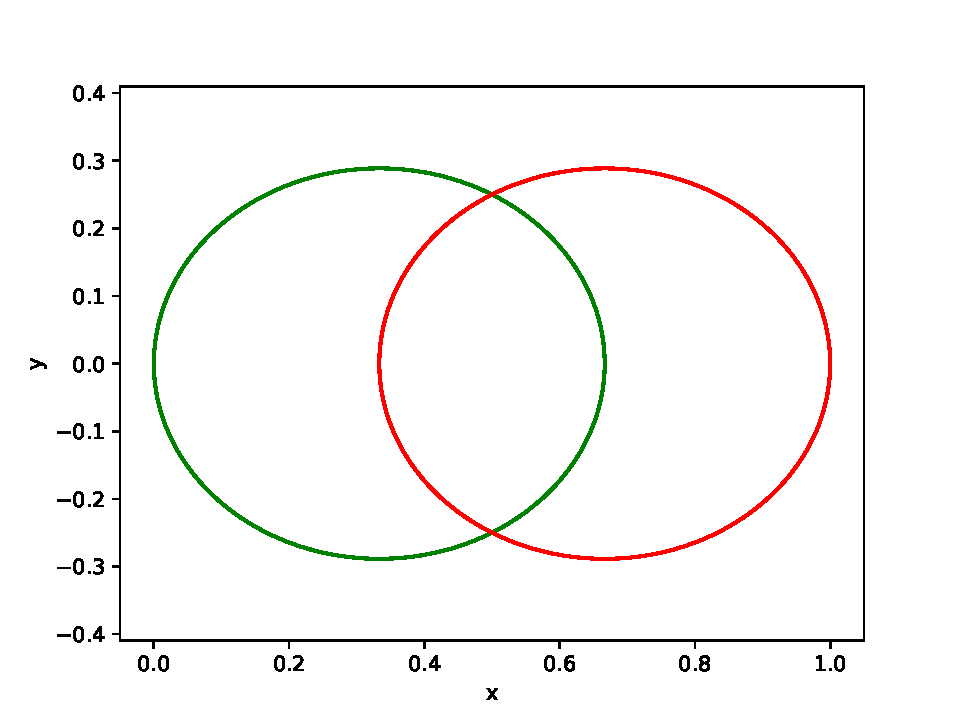
\includegraphics[width=6.5cm]{kreisoffset.pdf} 
    \caption{Offset orbits due to higher initial speed} 
\end{figure}

\subsection*{d)}
If we choose an initial velocity above \( \sqrt{2} v _{0} \), the gravitational
pull of the two objects becomes too tiny and the algorithm fails due to rounding
.

\subsection*{e)} 
Decreasing the time step size will result in a smoother curve and a better
approximation of the actual solution. The chance of rounding down the Force
gets smaller. Increasing the step size will result in bigger divergence and
the chance that the gravitational pull being rounded to 0 becomes higher, hence
resulting in the particles flying away from each other.

\section*{Problem 5 - Error Analysis of Euler Scheme}

We use our previous examples and calculate the eccentricity as well as the 
energy difference between initiation and the different steps.

\begin{table}[ht]
    \centering
    \begin{tabular}{lcc}
	\toprule 
	\( \Delta t \) & v\_0 & e \\ \midrule 
	\( 10 ^{-2} \) & \( 1/ \sqrt{2} \) & 0.963 \\
	\( 10 ^{-4} \) & \( 1/ \sqrt{2} \) & 0.714 \\
	\( 10 ^{-4} \) & \( 1/2 \) & 0.991 \\
    \bottomrule 
\end{tabular}
\end{table}

\begin{figure}[ht]
    \centering
    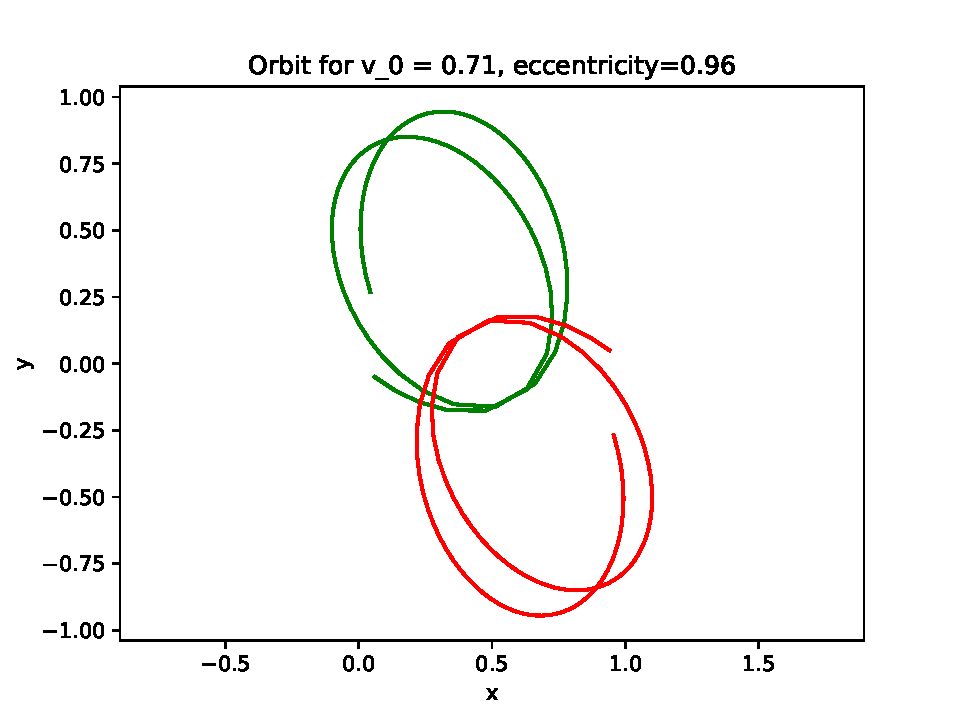
\includegraphics[width=7cm]{1.pdf} 
    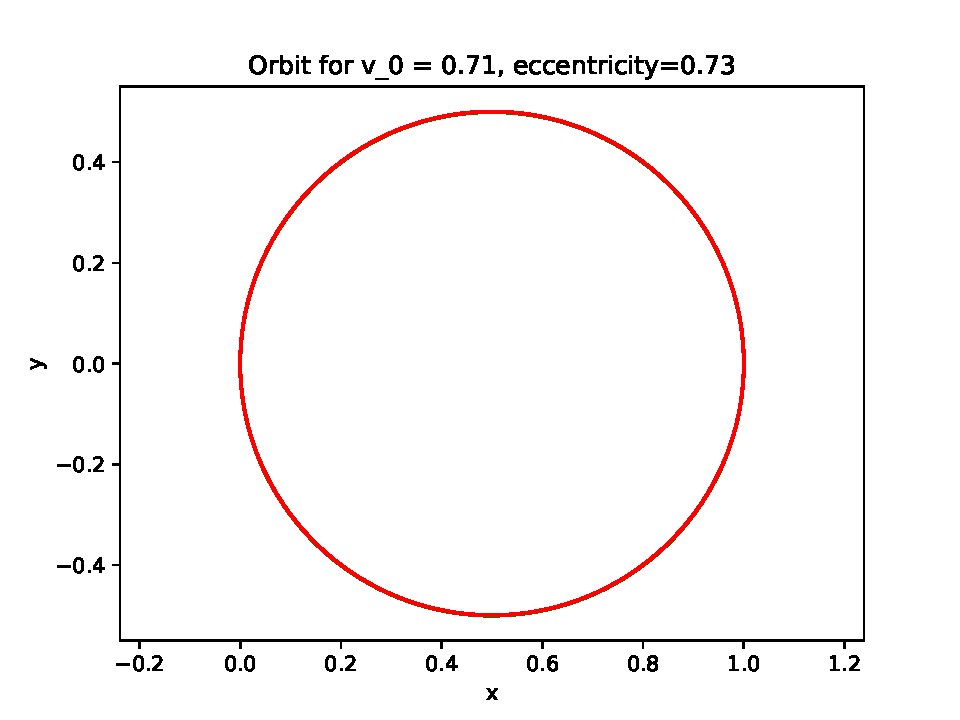
\includegraphics[width=7cm]{2.pdf} 
    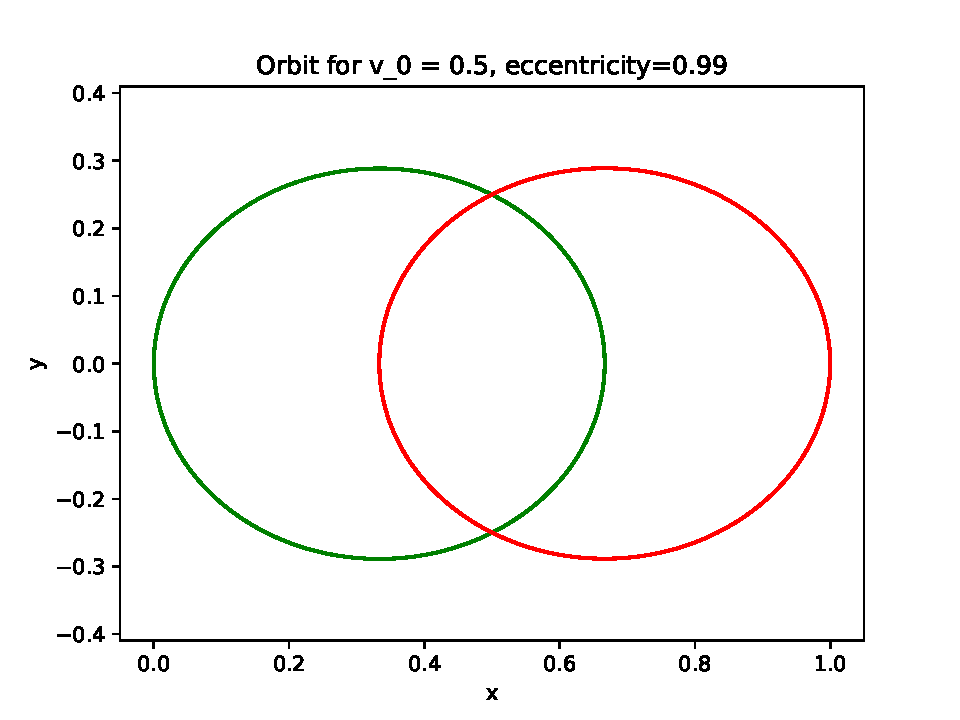
\includegraphics[width=7cm]{3.pdf} 
    \caption{Trajectories}
\end{figure}

\begin{figure}[ht]
    \centering
    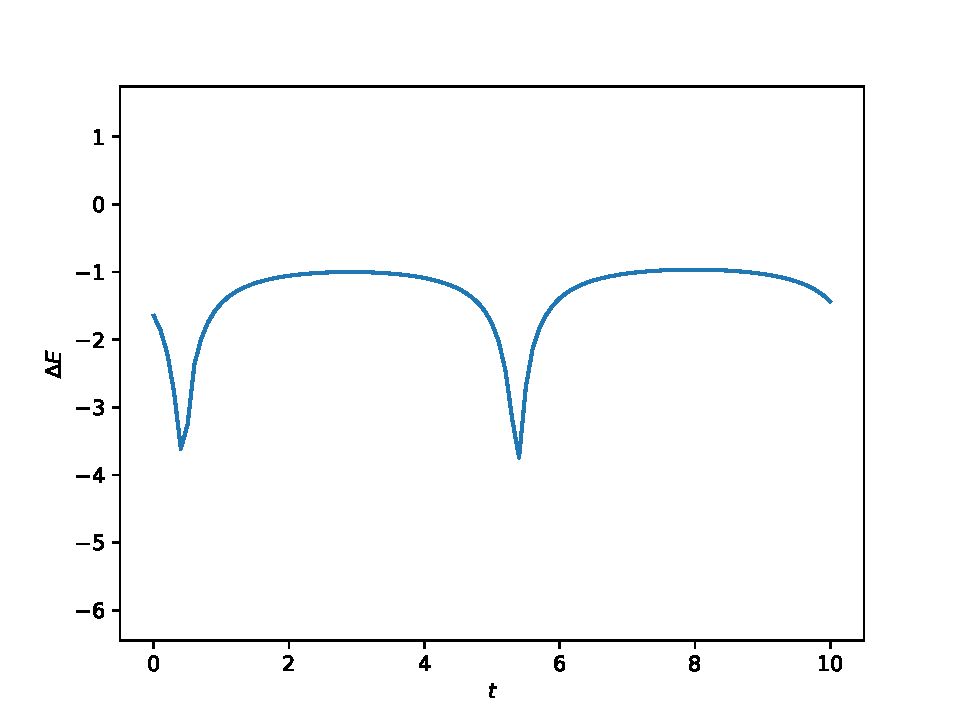
\includegraphics[width=7cm]{1e.pdf} 
    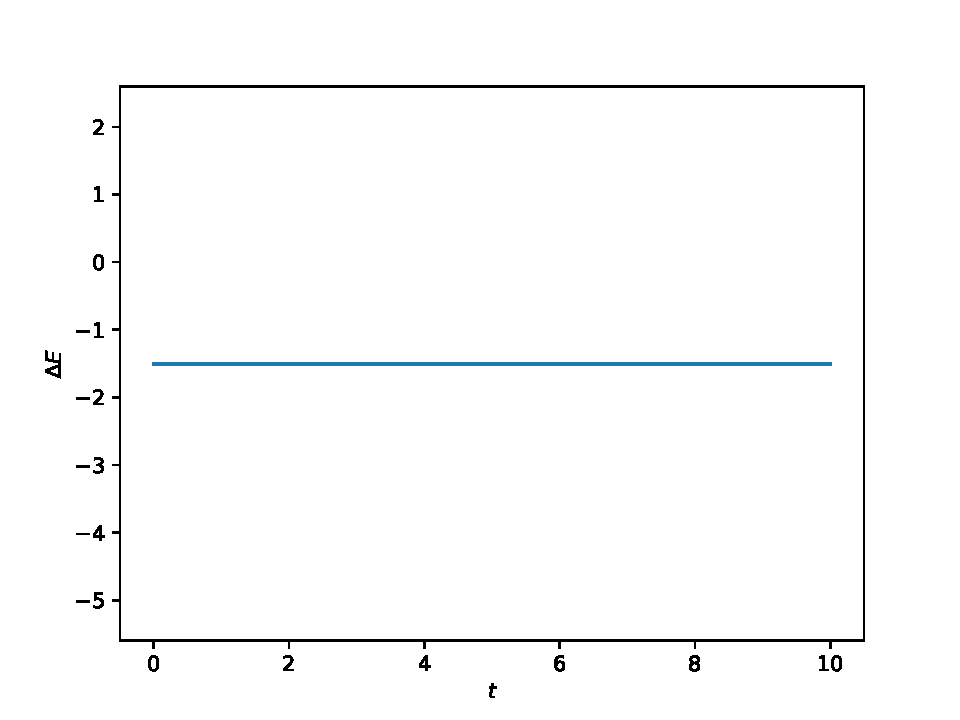
\includegraphics[width=7cm]{2e.pdf} 
    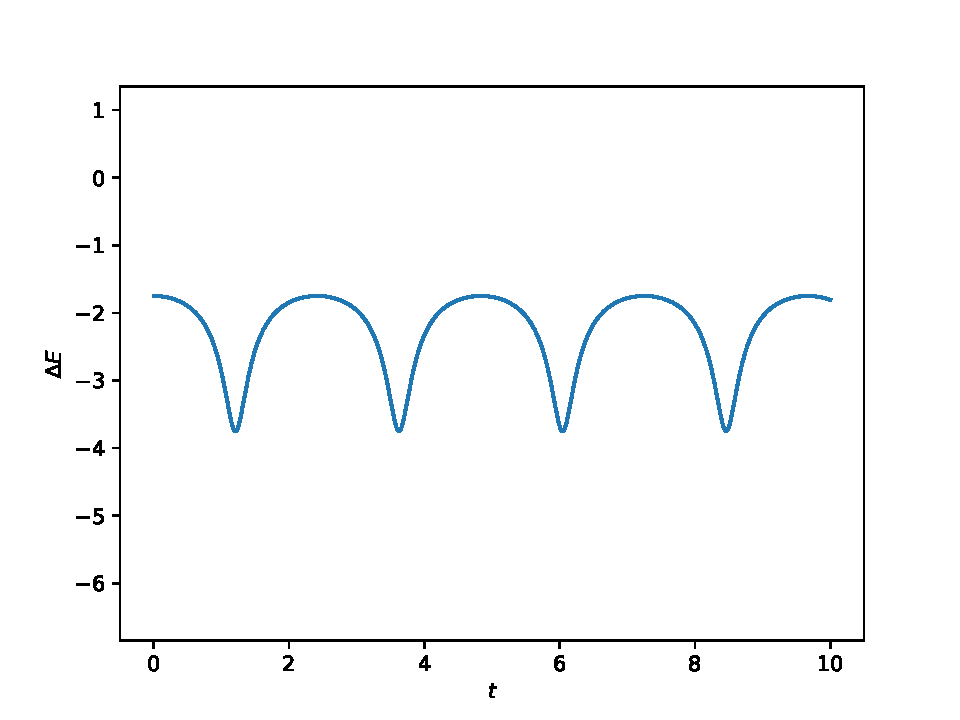
\includegraphics[width=7cm]{3e.pdf} 
    \caption{Energy differences}
\end{figure}

\end{document}

